%TODO schema evolution and versioning introduce two main problems: the semantics of changes, and the change propagation
%TODO podívat se na formulace v SERF
\documentclass[11pt]{article}
\usepackage{amssymb}
\usepackage[fleqn]{amsmath}
\usepackage{hyperref}
\usepackage{graphicx}
\usepackage{semantic}
\usepackage{caption}
\usepackage{subcaption}

\title{Refactoring of Software Using Relational Database}
\author{Ondrej Macek}

\begin{document}
\maketitle
\section{Introduction}
\label{sec:intro}
The evolution (change) of a software is a common issue during software development. It occurs from many reasons in all phases of software lifecycle. The evolution severity usually depends on number of changes which has to be made and on the number of affected software components. The focus of this paper is in data evolution context of software implemented in object oriented language using relational database. It means that the data evolution affect at least two software components: persistent objects (entities) and the database. The evolution is based on developer's point of view in this paper as it origins in the need to evolve code. This kind of evolution is straightforward in case there are no data stored in the database, because the database schema can be generated according to an evolved code, moreover some object-relational mapping (ORM) frameworks are able to process basic evolutionary transformation on database with stored data. The evolution of an software with ORM become more difficult when there are stored data and when the evolutionary scenario is more complex. The data migration to the new database schema is usually processed manually, which is expensive and error prone.

This paper shows how the code refactoring can be used as the source for data migration. The approach based on changes in code is useful in case when there is no model of database as it is derived directly from code. Next it can help developers to understand impact  of code changes on database. The formal description of code refactoring impact on database and stored data can help with construction of a standalone migration framework or evolutionary extension for existing ORM frameworks.

The paper is organized as follows: first the evolution of software is described in detail in Sec. \ref{sec:problem}, then the related work in presented in Sec. \ref{sec:related-work}. In Sec. \ref{sec:models} the models of software and database is provided together with a set of basic evolutionary transformations. The impact of code refactoring on database is discussed in Sec. \ref{sec:evolution}. Finally the applicability and limitations of the proposed solution is discussed in Sec. \ref{sec:case}.

\section{Problem Definition} 
\label{sec:problem}
% víc rozepsat o změnách a jak se jim bránit a kam tím směřujeme
\textbf{TODO: write an introduction when and why the software changes. and possible solutions.}
A software implemented using an object-oriented language, which uses relational database as a data storage (as illustrated in the Figure \ref{fig:evolution}) is object of interest of this paper. There are three important components of such a software: application (its persistent layer concretely), database (consisting of database schema and stored data) and an ORM, therefore we define a software as a triple consisting of an application and a database which are connected together by an ORM:
\begin{align*}
& \mathbf{software} = ( Application, Database, ORM )
\end{align*}
The software has to be in consistent state so its users could have benefit from its usage. The state of the software is defined to communicate the sate of the software to its user, the symbol $\perp$ is used as a notation for inconsistent state. 
\begin{align*}
& \mathbf{state} = Consistent\; s \: | \: \perp, s \in State 
\end{align*}
The software is in consistent state if application and database are consistent and the database structure corresponds to the application structure according to the ORM.

The evolution of a software is a transformation from one consistent state to another one. These states are called generations of the software and the function which changed the state of a software are called transformations. The evolution consists of change in application and in database as shown in the Figure \ref{fig:evolution}. 
\begin{figure}
\centering
	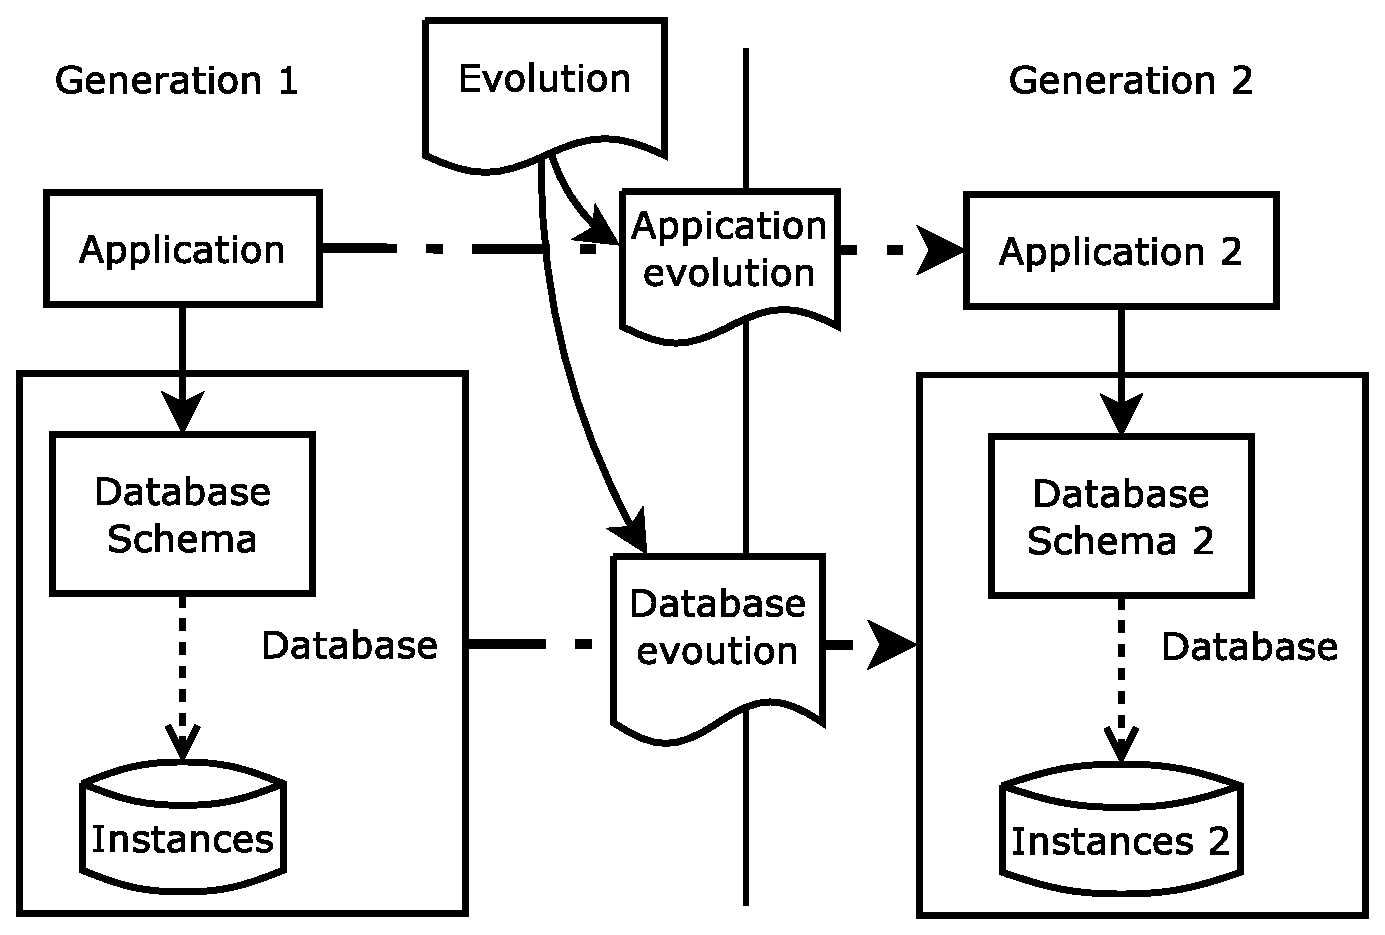
\includegraphics[scale=0.4]{./images/evolution_simple}
	\caption{The evolution of data changes the system on all levels. The figure shows all the components of the evolution process.}
	\label{fig:evolution}
\end{figure}
The usual approach is to refactor code (which is quite fast due to help of IDE) and then re-generation or manual migration of the database. Another approach is to evolve a database (e.g. due to database optimizations) and then update the code. This approach is very common too, nevertheless this paper focus on evolution which origin from the application point of view. 

The refactoring itself does not provide enough information for the complex migration of database and data, therefore a level defining the evolution is added - the set of all possible transformations $E$. The evolution definition from this level is propagated into both involved levels - application and database. The evolution is defined as:
\begin{align*}
& t(state(s)) = \begin{cases}
state(sw(\Psi(s, t), \Phi(s,t)) \; \mathbf{if} \; state(s) = Consistent \; s\\\\
 	\perp
\end{cases}\\ 
& s \in Software, t \in E
\end{align*}
Where $\Psi$ maps the software evolution cases to the code refactoring and $\Phi$ to maps to the evolutionary transformation of database.

The main issue during the software evolution is the preservation of data and information consistency. The data lost is a situation when data are damaged or lost during the migration. The information consistency means the data was transformed according to the evolution of the application and they correspond with developer's intention. 


\section{Related Work}
\label{sec:related-work}

\textbf{TODO}

\section{Model of Software}
\label{sec:models}
The aim of this paper is to provide an definition of data evolution, which can be applied in case of various programming language, therefore the platform independent models of application and database are introduced. These models also provide simplification, which should increase the understanding of the proposed evolutions.

\subsection{Application Model}
%TODO popis
\paragraph{Application} Application is defined as a sequence of classes and it creates the context for all structures used in the software persistent layer.
\begin{align*}
& \mathbf{Application} = (Class*)
\end{align*}

\paragraph{Class} Class represents a basic structural unit in the application model. It has a unique name, one or more properties and it can be associated to other classes in the application. 
\begin{align*}
& 	\mathbf{Class} = (label, Property*, Association*)
\end{align*}
The properties of a class can be of two kinds - values or collections - according of theirs cardinality.
	 
\paragraph{Property} Property represents a feature of a class which is represented as a primitive type. The property can be mandatory, can have a default value and according to its cardinality it can represent a single value or a collection of values. 
\begin{align*}
&	\mathbf{Property} = (label, AppType, DefaultValue, Cardinality, Mandatory)
\end{align*}

\paragraph {Association} Association represents a connection between two classes. It has a unique name and the reference is represented by the label of referenced class. The class which owns the association is consider to be the starting class of an association, referenced class is consider to be the ending class of an association. The cardinalities defines the multiplicity of both association ends.
\begin{align*}
&	\mathbf{Association} = (label, classRef, startCardinality, endCardinality) 
\end{align*}

\paragraph{Application type} Application type ($AppType$) represents primitive type in the application. There are usually defined types such as String, Integer, Boolean etc. in contrast there is only one type in our model, because we focus on structural and data changes and type casting operations are not important for us. The only $AppType$ type is called $APPSTRING$.
\begin{align*}
& \mathbf{AppType} = APPSTRING
\end{align*}

%TODO consistency

\subsubsection{Application Manipulation}
\label{sec:app-evolution}
The application model defines only the structure of an application thus there are defined transformation for its creating, altering and disassembling. Therefore the conditions for successful transformations are simple 1) when creating an object in the model or altering its name collisions has to be prevent, 2) when renaming a class the references have to be updated 3) when creating or altering an association the existence of referenced class has to be verified. The only issue during disassembling is the class can be removed only in case it is not associated by other classes. If a transformation cannot be processed the state of the application become inconsistent. The transformations are in table \ref{tab:app-evolution}. The list of altering operations is not complete as there are missing transformation for changing the obligation or cardinality of properties and associations. It is because these transformations are not so important for the next text when the complex refactorings are considered. 
\begin{table}
\centering
	\begin{tabular}{|l|}
	\hline
	\textbf{Application Creation} \\
	newProperty(className, property, application) \\
	newAssociation(className, association, mapping, application) \\
	newClass(class, application) \\
	\textbf{Application Alternation} \\
	renameProperty(className, oldName, newName, application) \\
	renameAssociation(className, oldName, newName, application) \\
	renameClass(oldName, newName, application)\\
	changeReference(referncedClass, newReferencedClass) \\
	\textbf{Application Disassembly} \\
	removeProperty(className, propertyName, application) \\
	removeAssociation(className, associationName, application) \\
	removeClass(className, application)\\
	\textbf{Copy Structure}\\
	copyProperty(sourceClass, property, targetClass, newName, application)  \\
	copyClass(class, newName, application) \\
	\hline
	\end{tabular}
	\caption{The transformations for application evolution.}
	\label{tab:app-evolution}
\end{table}

\subsection{Database Model}
he relational database consists of database schema which defines the structure of the database and data, which in our ORM system represents stored instances. The database is defined as a tuple:
\begin{align*}
&	\mathbf{Database} = ( Table*, Row* )
\end{align*}

\paragraph{Table} Table represents a basic concept of database schema. It has a unique name, one or more columns and it can be related to other tables in the schema by foreign keys. Rows in the table represents stored data.
\begin{align*}
&	\mathbf{Table} = (label, primaryKey, Column*, ForeignKey*)
\end{align*}

\paragraph{Column} Column defines data values and types which can be part of a table record.
\begin{align*}
&	\mathbf{Column} = (label, DbType, DefaultValue, Constraint*) 
\end{align*}

\paragraph{Foreign key} Foreign key is a reference to another table's primary key, it has an unique name and it can be constrained. The value of a foreign key is $\varnothing$ or a non-zero natural number.
\begin{align*}
&	\mathbf{ForeignKey} = (Label, Label, Constraint*) 
\end{align*}


\paragraph{Primary key} Primary key is unambiguous identifier of a record in a table. The primary key is always provided (automatically generated) by the database as a non-zero natural number. Primary key is always defined with constraints $NOTNULL$ and $UNIQUE$. 
\begin{align*}
&	\mathbf{PrimaryKey} =  ( Label, Sequence ) \end{align*}
The sequence generates values of primary key. The new value of a key is obtained by calling the function $next(s)$. The sequence which provides numbers incremented by one is called $s_1$ if the increment is 1, $s_{10}$ if the increment is 10 etc.

\paragraph{Data Types} Database data types $DbType$ represents primitive types in the database. There are usually defined types such as Varchar, Integer, Boolean etc. There is only one type of column values defined in the model called $DBSTRING$. Next the $DBINT$ type is defined for the values of keys.
\begin{align*}
&	\mathbf{DbType} = DBSTRING \; | \; DBINT
\end{align*}

\paragraph{Constraints} There are two types of constraints defined in the model. Both constraints are column constraints - first constraint defines non-empty columns, second constraint defines there has to be unique records in a column or foreign key.
\begin{align*}
&	\mathbf{Constraint} = NOTNULL \; | \; UNIQUE 
\end{align*}

A database consists not only from schema but also from data which are represented as rows in a table. A table row in our model is a tuple consisting of value pairs, which represents concrete value of concrete column or key. Each row contains a name of a table it belongs to.
\begin{align*}
&	\mathbf{Row} = (Label, N, Pair*) \\
&	\mathbf{Pair} = (Label, Value) 
\end{align*}

%TODO consistency

\subsubsection{Database Manipulation}
\label{sec:db-evolution}
The database consists of two parts - from database schema which defines the structure and from stored data - hence the transformations have to consider both parts. The transformation for manipualtion of structure has similar conditions to the evolution of application application. The transformations for data manipulation are inspired by the SQL language. The basic transformations are in Table \ref{tab:db-basic-evolution}. 
\begin{table}
\centering
	\begin{tabular}{|l|}
	\hline
	\textbf{Database Creation} \\
	addColumn(tableName, column, database) \\
	addForeignKey(tableName, key, database) \\
	addTable(table, database)\\
	\textbf{Database Alternation} \\
	alterColumnName(tableName, oldName, newName, dataabse) \\
	alterForeignKeyName(tableName, oldName, newName, dataabse) \\
	alterTableName(oldName, newName, dataabse) \\
	\textbf{Database Disasembling} \\
	dropColumn(tableName, columnName, database) \\
	dropForeignKey(tableName, keyName, database) \\
	dropTable(tableName, database) \\
	\textbf{Data Manipulation} \\
	select(tableName, rowId, database) \\
	select(tableName, database) \\
	insert(row, database) \\
	insert(rowId, value, database) \\
	delete(tableName, rowId, database) \\
	delete(tableName, rowId, columnName, database) \\
	\textbf{Copy Structure} \\
	copyColumnStructure(sourceTableName, targetTableName, \\  \hspace{0.5in} sourceColumnName, newName, database) \\
	copyTableStructure(sourceTable, newTableName, database) \\
	\textbf{Copy Strucutre and Values} \\
	copyColumn(sourceTable, targetTable, \\
	\hspace{0.5in} sourceColumnName, targetColumnName, \\ 
	\hspace{0.5in} mapping, database) \\
	copyTable(sourceTable, newName, database) \\
	\hline
	\end{tabular}
	\caption{The transformations for database evolution.}
	\label{tab:db-basic-evolution}
\end{table}
The set of transformations for database manipulation is limited in contrast with the SQL language it is because mentioned transformation are necessary for application of data evolution on database level. 

\paragraph{Copying of Database Elements} The transformations for copying the structure of a database elements serves more as helpers in advanced evolution cases as they adds a structural duplicate of an existing element only, nevertheless they are valid part of the transformation for database manipulation.  The copying of structural elements has the same limits as database creation - the transformation can not cause name collisions. 

The mapping between instances of the classes (stored data) to provides information which value from the source table rows will be copied to which row in target table. The value of a column is then inserted for each row into the copied column during $copyColumn$ transformation. 
The mapping is usually defined as: 
\begin{align*}
&	mapping =  (r_1, r_2)*,\\
& 	r_1 \in select(ORM(sourceName), database) \cup \varnothing, \\
& 	r_2 \in select(ORM(targetName), database) \cup \varnothing
\end{align*}
The mapping is not limited to the bijection and it is possible to not include a row into a mapping - this has to be verified because of possible $NOTNULL$ constraints on a target column, as well as the $UNIQUE$ constraint has to be verified because the mapping can violate it in general. On the other hand the benevolent mapping help with creating various kinds on advanced evolutionary transformations. The mapping can cause data losses in some cases if used as a part of advanced refactoring. This situation is discussed later on. 


\paragraph{Data Secure Disasembling of a Software} The transformation for disassembly the database can have fatal impact on the data preservation, therefore the set of transformations is extended by a data secure transformations for database disassembling. These transformations are not part of the SQL standard, although they can be implemented as database functions. These transformations creates a secure way to disassembly the database as they drops empty structural elements only. These transformations are in table \ref{tab:db-adv-evolution}. 
\begin{table}
\centering
	\begin{tabular}{|l|}
	\hline
	\textbf{Data Secure Database Disassembling} \\
	dropEmptyColumn(tableName, columnName, database) \\
	dropEmptyForeignKey(tableName, keyName, database) \\
	dropEmptyTable(tableName, database) \\
	\hline
	\end{tabular}
	\caption{The data secure transformations for database evolution which can be created as SQL functions.}
	\label{tab:db-adv-evolution}
\end{table} 



\subsection{Object Relational Mapping}
The ORM can differ from application to application, its impact on the evolution is not crucial but it has to be present to provide full information about the method. The mapping is similar to the Hibernate
mapping, thus a lot of developers should be familiar with it. 
% add mapping

\textbf{TODO: Describe ORM}

\subsection{Software Evolution}
\label{sec:sw-evolution}
The evolution of the whole software consider its both components application and database containing data. The way how evolutionary transformation are created based on the set of component specific transformations is introduced in this chapter.

The evolution is described from the developer point of view, therefore the transformations use the names and elements from application context. The names of application elements and elements themselves have to be transformed into a database context - this is assured by the ORM.

%Finally the evolution cases and their mappings on application and database components are presented in \ref{sec:sw-evolution}. 

%TODO evalutation of trnasformations

\subsection{Basic Evolutionary Transformations}
\label{sec:sw-basic-evolution}
The evolution of the whole software is based on the atomic transformations specific for each software part, which are defined in Sec. \ref{sec:app-evolution} and \ref{sec:db-evolution}. This section introduces how these primitives can be used to manipulate the software elements.

\paragraph{Basic Software Evolution} The basic evolutionary transformations of the software are based on basic evolution of an application. These transformation cannot be  mapped directly on the evolutionary transformations of the database, because properties and associations can be mapped as a column (foreign key respectively) or as a table, this has to be reflected during the evolution as shown on the example of creating a new property: 
\begin{align*}
& \Phi(newProperty(className, property, application)) = \\
& \;\;\; = \begin{cases}
  addColumn(ORM(className), ORM(property), database) \\\mathbf{if} \; cardinality(property \leq 1)  \\\\
  addTable(ORM(property), database) \\
  \mathbf{if} \; cardinality(property > 1)  
 \end{cases}
\end{align*}

Mapping between basic evolutionary transformations is provided in the shortened way in table \ref{tab:sw-basic-evolution}, there is the basic application transformation and possible mappings on database level according to to the cardinality.  

\begin{table}
\centering
	\begin{tabular}{|p{0.4\textwidth} p{0.5\textwidth}|}
	\hline
	Application Transformation & Database Transformation \\
	\multicolumn{2}{|c|}{\textbf{Software Creation}} \\
	newProperty & addColumn  ($cardinality \leq 1$)\\
	& addTable \\ 
	& \\
	newAssociation & addColumn ($cardinality \leq 1$)\\
	& addTable \\
	& \\
	newClass & addTable \\
	\multicolumn{2}{|c|}{\textbf{Application Alternation}} \\
	renameProperty & renameColumn ($cardinality \leq 1$)\\
	& renameTable \\
	& \\
	renameAssociation & renameForeignKey ($cardinality \leq 1$)\\
	& renameTable \\
	& \\
	renameClass & renameTable \\
	\multicolumn{2}{|c|}{\textbf{Application Disassembly}} \\
	removeProperty & removeColumn ($cardinality \leq 1$)\\
	& removeTable \\
	& \\
	removeAssociation & removeForeignKey ($cardinality \leq 1$)\\
	& removeTable \\
	& \\
	removeClass & removeTable\\
	\hline
	\end{tabular}
	\caption{The mapping between evolution of the application to the database transformations.}
	\label{tab:sw-basic-evolution}
\end{table}





The data secure transformations for disassembling the database can succeed (e.g. drop a table) when there are no data contained within the dropped element.


\subsection{Advanced Evolutionary Transformations}
\label{sec:sw-adv-evolution}
Advanced evolutionary transformations are based on the basic ones, they can be obtained as a concatenation of transformations. The concatenation of transformation is possible because each transformation produces a state of a software (or application or database) which can be used as an input for the next transformation. 

All transformations presented so far has the same input information for both application and database, whereas the advanced transformations usually needs a mapping between stored data (instances) as theirs input. 

\paragraph{Copy Property}
The $copyProperty$ creates a duplicate of a property in a given class. It can rename the property so it can be used for creating duplicates of a property in the property owning class. If the mapping is not provided the transformation creates only a structural copy of the property otherwise it copies the values too. Therefore the  $copyProperty$ transformation is the simplest way to manipulate stored data.

The  $copyProperty$ is the first transformation when an additional information has to be added to the usual code refactoring. It is because the $copyColumn$ transformation needs one more information to succeed - there has to be provided mapping between the source and target table to assure the data information consistency. %Moreover the source and target should have the same structure, type and constraints.
\begin{align*}
& \mathbf{copyProperty}(sourceClass, propertyName, targetClass, \\
& \; \; \; mapping, software) 
\end{align*}
The transformation is interpreted for both software components - in case of the application a new property is added:
\begin{align*}
& \Psi(copyProperty(sourceClass, property, targetClass, mapping, \\ 
&  \; \; \; software)) = newProperty(targetClass, property, application) 
\end{align*}
in case of database the copy of a column or table is created according to property's cardinality and then values are copied:
\begin{align*}
& \Phi(copyProperty(sourceClass, property, targetClass, newName,  \\ 
&  \; \; \; mapping, software)) = \begin{cases}
 coypColumn(ORM(sourceClass),  \\ \;\;\; ORM(targetClass),  \\ \;\;\;alterColumnName(ORM(property), \\ \;\;\; ORM(newName)), mapping, database) \\ \; \mathbf{if} \; cardinality(property) \leq 1 \\\\
 copyTable(ORM(Property), \\ \;\;\; ORM(newName))
 \end{cases}
\end{align*}

If there are no data in the target table an identity can be used as a mapping function instead of mapping above. 

\paragraph{Move Property}
The $moveProperty$ transformation is based on the $copy$ $Property$ transformation followed by the $removeProperty$ so its construction is easy. On the other hand special attention has to be paid to the provided mapping of instances, because it can cause data loses. The ideal case is when the mapping is a bijection among instances, then the transformation can not cause the lost of data. On the other hand the situation when the mapping does not provides pairs for all rows in a source table can lead to data loss. 
\begin{align*}
& moveProperty(sourceClass, property, targetClass, newName, \\
& \;\;\; mapping, software) = removeProperty(sourceClass, property, \\
& \;\;\; CopyProperty(sourceClass, property, targetClass, \\ 
& \;\;\;newName, mapping, software))
\end{align*}

\paragraph{Merge Classes}
There occur situations when there is a need to merge two classes and the inlining transformation cannot be used because of name collisions among properties in such a case the $merge$ transformation can be used. It can be used in case structure of both classes (respectively tables) are equal. The transformation creates new rows in the new table - the primary keys from origin instances are replaced by a new ones.
\begin{align*}
& merge(firstClass, secondClass, newClassName, software) = \\
& \; \; \; = removeClass(secondClass, removeClass(firstClass, \\
& \; \; \; changeReference(secondClass, newClassName, \\
& \; \; \; changeReference(firstClass, newClassName, \\
& \; \; \; copyClass(firstClass, newClassName, software))))))
\end{align*}


\paragraph{Extract and Inline Class}
The extract and inline class are two opposite transformations. First of them extract a class from an existing class, second of them moves data from one class into another.
\begin{align*}
& extract(sourceClass, newClass, property*, software) = \\ 
& \; \; \; = moveProperty(sourceClass, newClass, property*, \\ 
& \; \; \; addClass(newClass, software))
\\\\
& inline(targetClass, classToInline, software)) = \\
& \; \; \; = removeClass(classToInline, moveProperty(classToInline, \\
& \; \; \; targetClass, properties(classToInline), software))
\end{align*}

The advanced refactoring cases are limited by the transformations they are created from.

\section{Case Study}
\label{sec:case}
It is obvious that the set of defined transformation is limited because of focus on data preservation or transformation concatenation. On the other hand defined transformations are strong enough to handle a lot of refactoring cases. 

Before one complex case study example is shown a set of small refactoring cases is discussed. These cases are chosen based on the Eclipse foundation refactoring statistics (the transformation from the top ten influencing data chosen only) and on Martin Fowler's book: Refactoring - improving design of existing code, where one chapter is dedicated to the data organization in the software. 

Selected refactorings are:
\begin{enumerate}
	\item \textbf{Rename} is the most used refactoring used according to Eclipse statistic and it is one of the basic refactoring cases introduced in the Sec. \ref{sec:sw-basic-evolution}.
	\item  \textbf{Move} refactoring is used in Eclipse to move properties from a class to another class within an inheritance hierarchy or to move classes between packages. In contrast our model does not consider packages, on the other hand it is able to move property from one class to another according given mapping, which contains not only move in hierarchy but a lot of other cases too.
	\item \textbf{Extract Class} is often used refactoring in Eclipse and it is mentioned in Fowler's book too. It is introduced as an example of advanced refactorings in Sec. \ref{sec:sw-adv-evolution} together with its opposite transformation $inline$.
	\item \textbf{Move field} from the Fowler's book is introduced as $moveProperty$ in Sec. \ref{sec:sw-basic-evolution}.
	\item \textbf{Replace Data Value with Object} is a refactoring case which is not mentioned among the evolutionary transformations, on the other hand it can be composed from already defined transformations:
	\begin{align*}
& replaceDataWithObject(sourceClass, property, newObject, \\
& \; \; \; software) = removeProperty(sourceClass, property, \\
& \; \; \; newAssociation(sourceClass, newObject,  mapping, \\
& \; \; \; copyProperty(sourceClass, property, newObject, \\ & \; \; \;  software)
	\end{align*}
Where the mapping use the values copied in the first transformation as a matching point for creating connection between the old and the new class.
\end{enumerate}
The transformations proposed in this paper are able to implement all data refactorings used on Eclipse platform. There are some refactorings from Fowler which are not considered in the proposal: replace array with object, change unidirectional association to bidirectional (and reverse) and operations which replace types with polymorphism.

\subsection{Example of Usage}
The example demonstrates how the transformation helps with data evolution in real example of software evolution. There are two classes in our software $Person$ and $LegalParty$ both of them contains information about address (street, city and zip code). The situation in software is in Figure \ref{fig:case1}, where the whole software is shown. 

To improve the design of code the class Address has to be created which associated with both original classes and contains the data already stored in the software. 
\begin{figure}
\begin{subfigure}[b]{0.45\textwidth}
	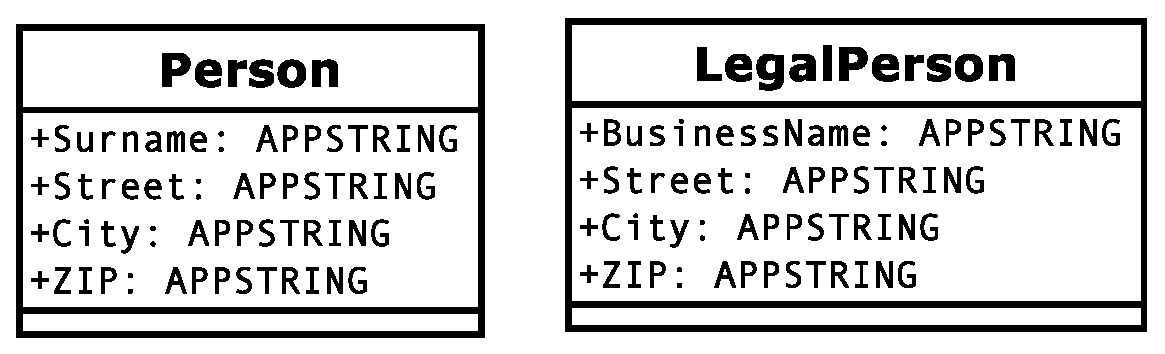
\includegraphics[width=\textwidth]{./images/case_app_1}
	\caption{The application model.}
\end{subfigure}
\quad
\begin{subfigure}[b]{0.45\textwidth}
	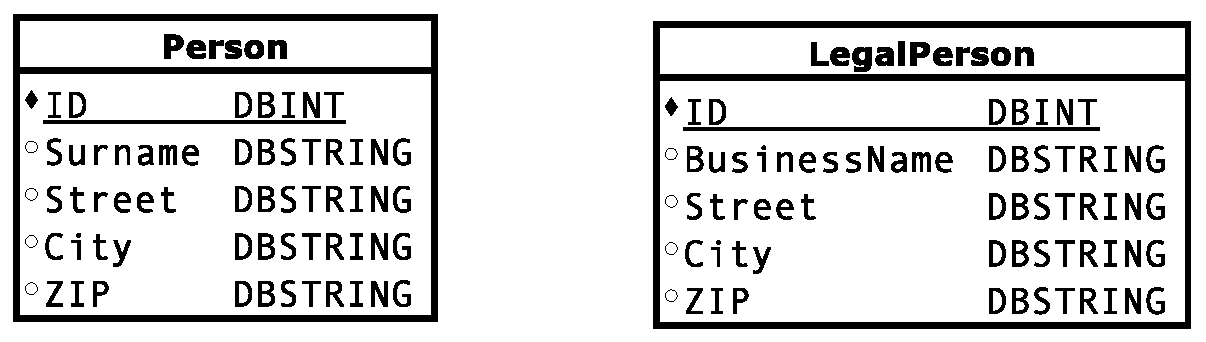
\includegraphics[width=\textwidth]{./images/case_db_1}
	\caption{The database model.}
\end{subfigure}
\begin{subfigure}[b]{\textwidth}
	\centering
	\begin{tabular}{| c | l | l | l | l | }
	 	\hline
		Id &  Surname & Street & City & ZIP  \\ \hline  
		11 & Jackson & Central Park St & New York & 100 01  \\ \hline
		12 & Clooney & S Orange Ave & Orlando & 320 24  \\ \hline
	\end{tabular}
	\caption{Data stored in the table $Person$.}
\end{subfigure}
\begin{subfigure}[b]{\textwidth}
	\centering
	\begin{tabular}{| c | l | l | l | l | c |}
	 	\hline
		Id &  BusinessName & Street & City & ZIP \\ \hline  
		100 & Tools \& Machines & Olive ave. & New York & 100 01 \\ \hline
		200 & AI Robotics & Pine ave. & LA & 900 03  \\ \hline
	\end{tabular}
	\caption{Data stored in the table $LegalParty$.}
\end{subfigure}
	\caption{The initial state of the example used in the case study. There is a repetition of information structure in the $Person$ and $LegalParty$ class.}
	\label{fig:case1}
\end{figure}
The first  step of is to extract two temporary classes representing address of a $Person$ or of a $LegalParty$. Temporary classes has to be connected with the origin classes by an association.
\begin{align*}
 s' &= merge("Address\_tmp1", "Address\_tmp2", "Address", \\
& \;\;\;\;  newAssociation("LegalParty", association("address", \\
& \;\;\;\; "Address\_tmp2", 1, 1), mapping_2, extract("LegalParty", \\
& \;\;\;\;  "Address\_tmp2", "street", "city", "zip", \varnothing  \\
& \;\;\;\; newAssociation("Person", association("address", \\
& \;\;\;\; "Address\_tmp1", 1, 1), mapping_1, extract("Person", \\
& \;\;\;\; "Address\_tmp1", "street", "city", "zip", \varnothing, software)))
\end{align*}
Both $mapping_1$ and $mapping_2$ are identities so the creation of the association is straightforward. The result of the transformations is in the Fig. \ref{fig:case2}. 
\begin{figure}
\begin{subfigure}[b]{0.45\textwidth}
	\centering
	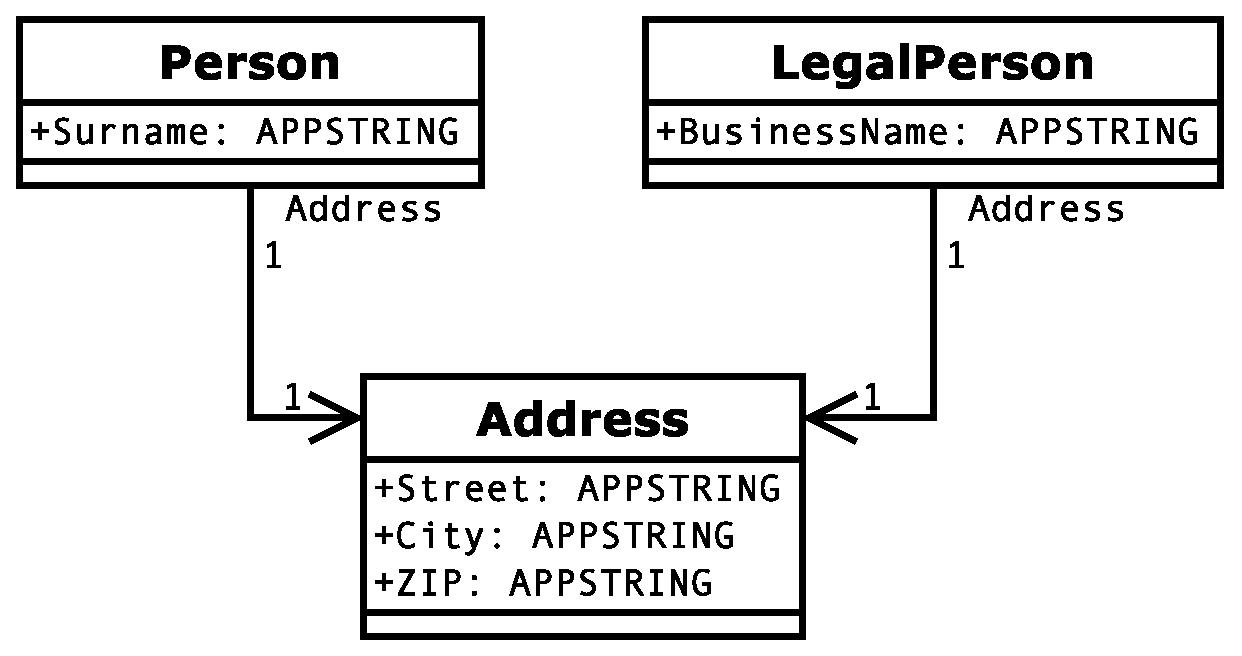
\includegraphics[width=\textwidth]{./images/case_app_9}
	\caption{The application model.}
\end{subfigure}
\quad
\begin{subfigure}[b]{0.45\textwidth}
	\centering
	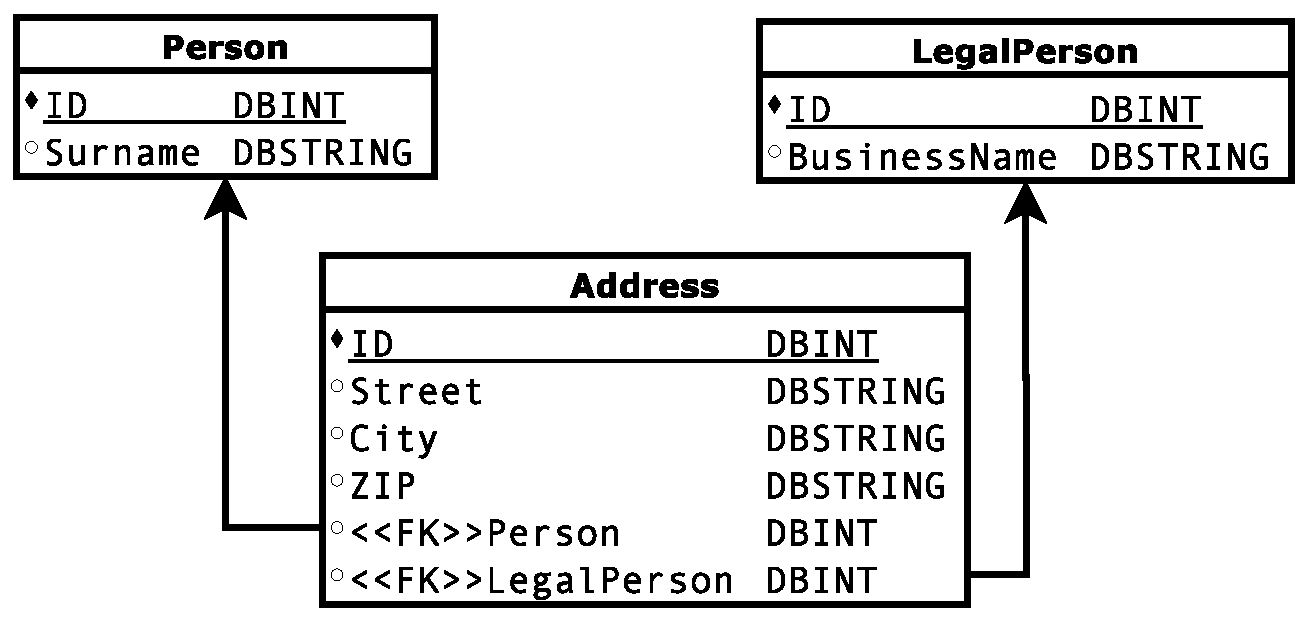
\includegraphics[width=\textwidth]{./images/case_db_8}
	\caption{The database model.}
\end{subfigure}

\begin{subfigure}[b]{0.5\textwidth}
	\centering
	\begin{tabular}{| c | l |}
	 	\hline
		Id &  Surname \\ \hline  
		11 & Jackson  \\ \hline
		12 & Clooney  \\ \hline
	\end{tabular}
	\caption{Data stored in the table $Person$.}
\end{subfigure}
\begin{subfigure}[b]{0.5\textwidth}
	\centering
	\begin{tabular}{| c | l |}
	 	\hline
		Id &  BusinessName  \\ \hline  
		100 & Tools \& Machines  \\ \hline
		200 & AI Robotics \\ \hline
	\end{tabular}
	\caption{Data stored in the table $LegalParty$.}
\end{subfigure}
\begin{subfigure}[b]{\textwidth}
	\centering
	\begin{tabular}{| c | l | l | l | l | l |}
	 	\hline
		Id & Street & City & ZIP & Person\_Address & LegalParty\_Address\\ \hline  
		1 & Olive ave. & New York & 100 01 & & 100 \\ \hline
		2 & Pine ave. & LA & 900 03 & & 200  \\ \hline
		3 & Central Park St & New York & 100 01 & 11 &  \\ \hline
		4 & Orange Ave & Orlando & 320 24 & 12 &\\ \hline
	\end{tabular}
	\caption{Data stored in the table $Address\_tmp2$.}
\end{subfigure}
	\caption{The initial state of the example used in the case study. There is a repetition of information structure in the $Person$ and $LegalParty$ class.}
	\label{fig:case2}
\end{figure}

The example shows that defined transformations are able to perform regular data evolutions. It shows that usage of the transformations are sometimes not intuitive for user (e.g. creating temporary classes before merge).


\section{Conclusion}



\end{document}
